%!TEX root = thesis.tex
%=============================================================================

\section{Robocup Speech Recognition Test}
In this section, an evaluation of the proposed pipeline in a real work scenario will be presented.
The goal of this evaluation is to evaluate if using the proposed pipeline leads to improved recognition results, in this particular case to better sound source localization results.

This evaluation will be based on the Speech \& Person Recognition task of RoboCup@home 2018 \cite{speechrec_2018}, although some minor modifications will be made to the setup.
The evaluation will be conducted on the Pepper robot (TODO cite).

\subsubsection{Software Setup}
Two distinct solutions will be benchmarked:
The existing RoboCup setup and a reimplementation of it within the proposed pipeline.
Both will mainly be comprised of a sound source localization, a speech recognizer and a layer to combine the results of both these components.

The proposed pipeline (see figure \ref{pic:eval_task_setup_new}) will consist mainly of the basic speech recognition setup established as the baseline for the dataset evaluation (see chapter \ref{eval:dataset:pipeline:baseline}), i.e. an audio grabber to record audio from a microphone as well as the previously (see chapter \ref{eval:dataset:setup}) established VAD, PocketSphinx speech recognizer and Orchestrator.
As sound source localization a component using pyroomacoustics, and specifically, its SRP algorithm, will be employed.
Due to the robot providing four channel audio from its four microphones, which are all needed by the SSL, but the speech recognition part of the pipeline requiring only one channel audio, an additional component is needed in the form of a channel splitter.

For the existing solution (see figure \ref{pic:eval_task_setup_old}), the already established PSA will take the role of the speech recognizer.
For sound source localization, a slightly modified variant of the proposed pipelines component will be employed.
To combine both results, an established behavior controller called Bonsai (TODO: cite bonsai) will be used.
An channel splitter as with the proposed pipeline is not necessary, as ALSA will assume this task for the PSA.

Of course, similar components within both solutions will be equivalently configured.
The logged output of both solutions will contain SSL angles and recognized speech.
Both solutions will be run concurrently, to eliminate run-to-run variances between the solutions.


\subsubsection{Modification to the RoboCup@home task}



\subsubsection{Robocup task setup and modifications}
- 5-10 runs are planned

-Extensive noise is generated around the robot, to simulate a crowded convention center

-Simultaneous execution of both solutions require small changes to the task

-Since the robot can not turn to two different angles at once, logged angle information will be used to evaluate SSL results

-For similar reasons and since producing answers to the questions can be done rather easily, recognizing the correct question will count as correctly answered

-The person recognition part of the task is irrelevant for this evaluation and will be left out. The task will instead start with the ''riddles'' game

-To ease the evaluation of SSL results, only four persons will partake in the ''blind mans bluff'' game. One person each will stand directly in front of the robot, behind the robot and to either side of the robot, with a 90$^\circ$ shift in angle with respect to the initial orientation of the robot

- The existing RoboCup setup (PocketSphinxAdapter, pyroomacoustics SSL) will run on the robot

-The proposed pipeline (PocketSphinx node, re-implementation of PocketSphinxAdapter VAD, pyroomacoustics SSL) will run on a secondary machine (except for a audio grabber node, which must run on the robot)

-Questions for the task will be generated from the publicly available RoboCup 2018 command generator

-Noise will be generated via a handful of evenly distributed speakers playing restaurant noises (mostly human chatter) in a big, echoing place (i.e. in front of Citec lecture hall)

-Task will be carried out as described in RoboCup@home Rulebook 2018, apart from above modifications

-Both PocketSphinx implementations will use the same grammar, dictionary and speech-model needed for the task

\subsubsection{Goal}
-Evaluating SSL results. Pinpoint accuracy is not required. Rather erroneous detections caused by noise before or after the spoken question should not occur. As such, any SSL result within a margin of error of +-15$^\circ$  can be regarded as correct. 

-Word error rate/ percentage of correctly understood questions can be used as a control variable 

\subsubsection{comparability}
-Both SSL solutions are virtually identical (apart from the fact that the RoboCup setup one will grab audio directly from the microphones and the one from the proposed pipeline will use audio transmitted via said pipeline)

-The VAD used in the proposed pipeline is a direct re-implementation of the VAD used in the PocketsphinxAdapter

-Both pipelines use Pocketsphinx for speech recognition, PocketSphinxAdapter uses the c/c++ interface, the PocketSphinx node of the proposed pipeline uses the official python wrapper

-Why not run independently? 

-Does the re-implementation make a difference?

-Can you automate this instead of using ppl?

-Noise must always be the same?


\subsubsection{evaluation of results}


\begin{itemize}
	\item oftentimes recognition results would be very similar, but once wrong and once right, e.g. ''whats the color of the coke'' would be once interpreted by both pipelines as ''whats the color of the bowl'' and once by the old pipeline as ''whats the color of the fork'' and once correct by the proposed pipeline; other example: sponge was recognized as sausages, thus once wrong
\end{itemize}

\subsection{Discussion}


\begin{figure}[]
	\centering
	\subfloat[Scenario for baseline of proposed pipeline]{
		\includegraphics[width=0.5\textwidth]{diagrams/robocup_task_t.pdf}
	}
	\subfloat[Scenario for elongated baseline of proposed pipeline]{
		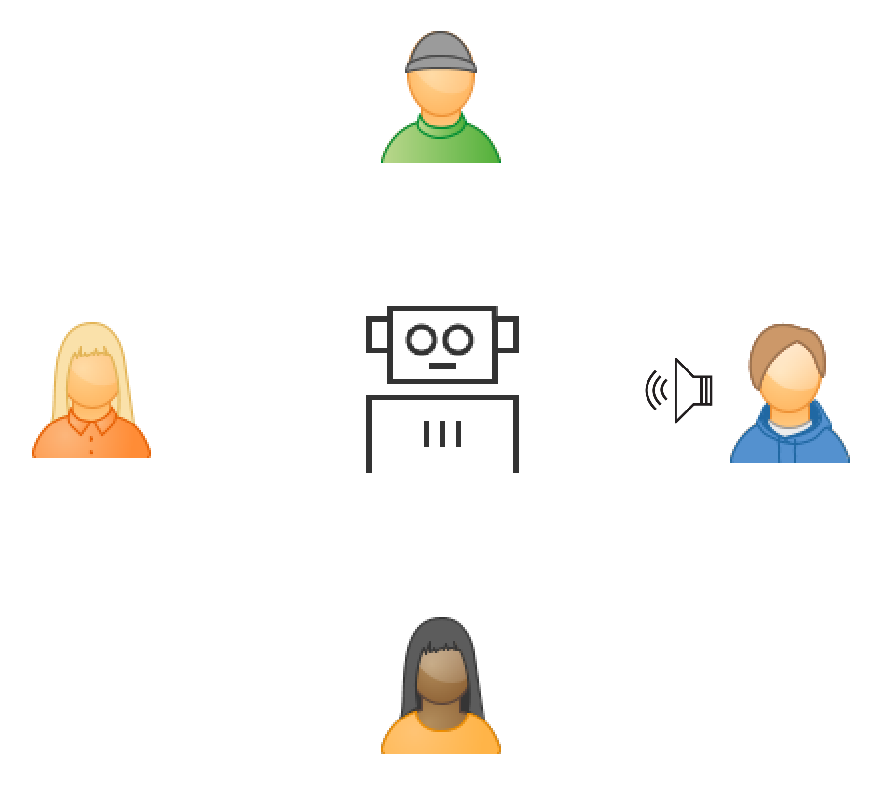
\includegraphics[width=0.5\textwidth]{diagrams/robocup_task_t1.pdf}
	}
	\caption{Test scenario for the RoboCup task}
	\label{pic:eval_task}
\end{figure}

\begin{figure}[]
	\centering
	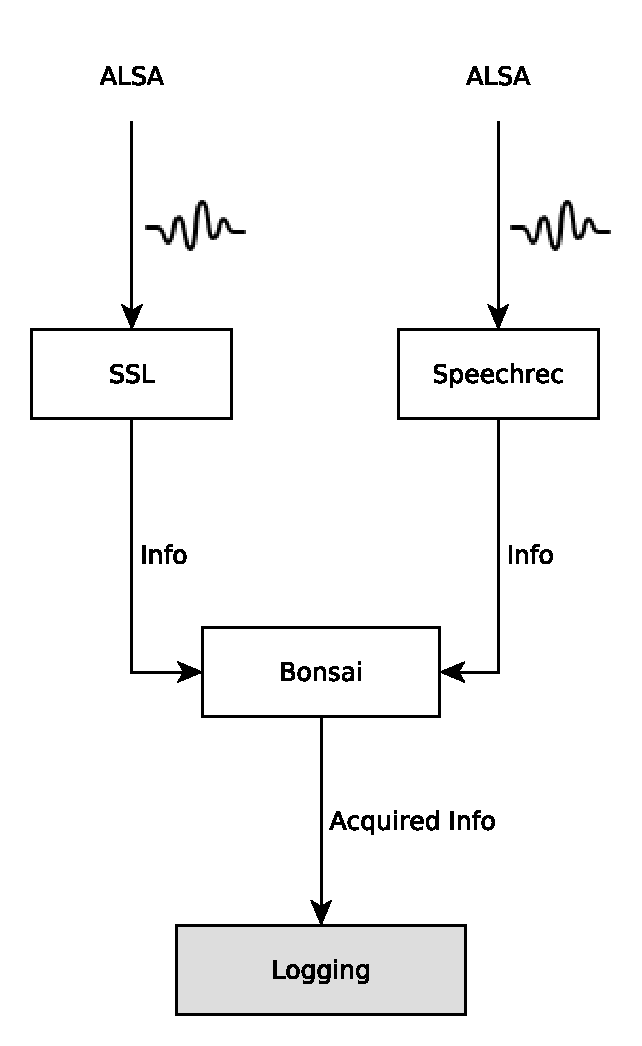
\includegraphics[width=0.5\textwidth]{diagrams/eval_task_old.pdf}
	\caption{Setup of existing solution}
	\label{pic:eval_task_setup_old}
\end{figure}

\begin{figure}[]
	\centering
	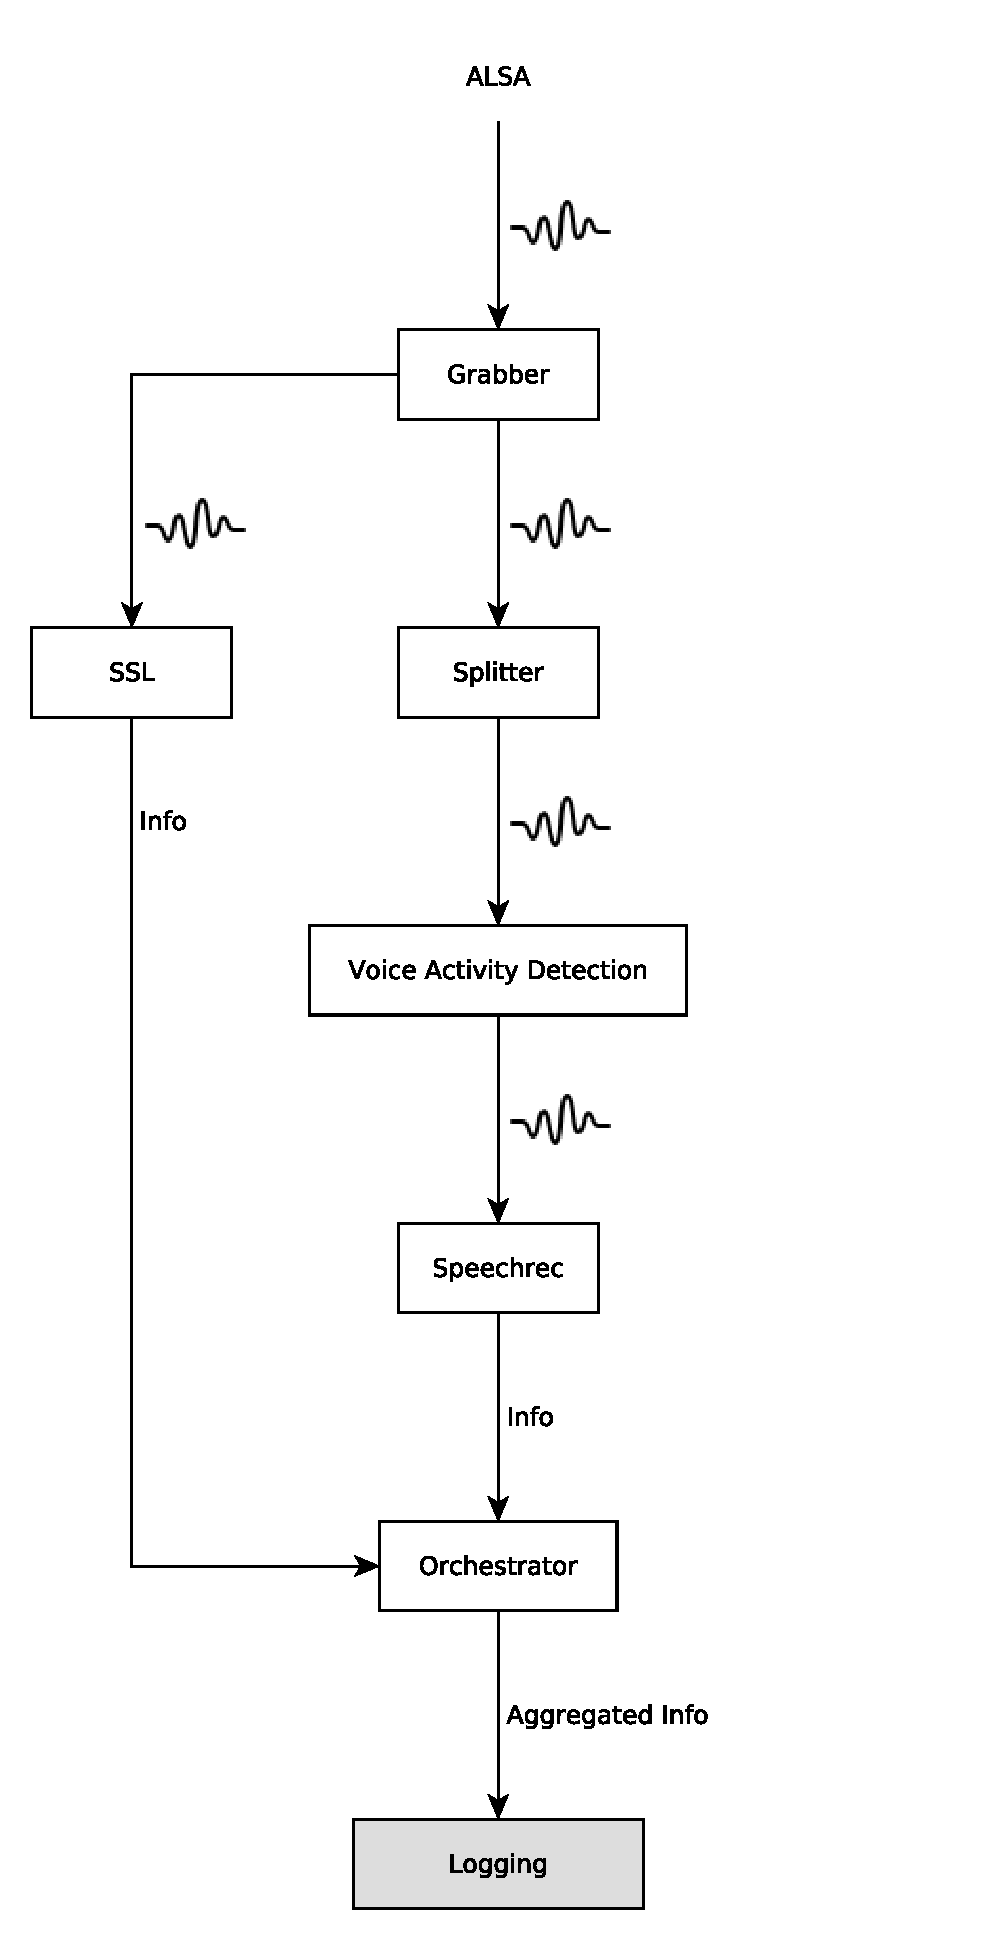
\includegraphics[width=0.5\textwidth]{diagrams/eval_task_proposed.pdf}
	\caption{Setup of of proposed pipeline}
	\label{pic:eval_task_setup_new}
\end{figure}

\begin{figure}[]
	\begin{tabular}{ | l | l | l | l |}
		\hline
		Run & Correctly recognized sentences & Points & Points by SSL \\ \hline
		1 & 50\% & 45 & 0 \\ \hline
		2 & 50\% & 40 & 10 \\ \hline
		4 & 35\% & 25 &  0 \\ \hline
		5 & 40\% & 30 & 10 \\ \hline
		6 & 45\% & 40 & 10 \\ \hline
		7 & 60\% & 50 & 10 \\ \hhline{|=|=|=|=|} 
		Avg & 46.7\% & 38.3 & 6.7 \\
		\hline
	\end{tabular}
	\caption{Results of the existing pipeline in the RoboCup task}
	\label{pic:eval_task_results_old}
\end{figure}

\begin{figure}[ht]
	\begin{tabular}{ | l | l | l | l |}
		\hline
		Run & Correctly recognized sentences & Points & Points by SSL \\ \hline
		1 & 65\% & 50 &  0 \\ \hline
		2 & 55\% & 70 & 20 \\ \hline
		4 & 55\% & 35 &  0 \\ \hline
		5 & 55\% & 50 & 20 \\ \hline
		6 & 60\% & 60 &  0 \\ \hline
		7 & 60\% & 60 & 10 \\ \hhline{|=|=|=|=|} 
		Avg & 58.3\% & 54.2 & 8.3\\
		\hline
	\end{tabular}
	\caption{Results of the proposed pipeline in the RoboCup task}
	\label{pic:eval_task_results_new}
\end{figure}